\chapter{Introduction}

\section{Objectif du projet}

Le but de ce projet est de découvrir une nouvelle technologie concernant l'automatisation, le
déploiment, le clustering ou encore le cloud. Cela nous permettra de découvrir différents outils
que l'on sera peut-être amené à manipuler dans le futur.

\section{Présentation de la technologie}

\subsection{Docker}

\columnratio{0.6}
\begin{paracol}{2}

Docker est un outil open-source, sorti en 2013, permettant de concevoir, tester et déployer
rapidement des applications. Il utilise la notion de conteneurs qui, comme la virtualisation,
permet d’isoler une application de la machine hôte tout en étant plus léger et plus simple à
déployer.

\switchcolumn


\includegraphics[width=0.7\linewidth]{img/docker}

\end{paracol}
\jmp

Docker étend les conteneurs \emph{LXC (Linux Container)} qui s’appuient sur les fonctionnalités du
noyau pour l’isolation (namespaces, cgroups), en fournissant une API haut niveau, plus simple
d’utilisation.\newline

Comme on peut le voir sur la figure \ref{fig:diffvm}, la différence principale entre un conteneur 
et une machine virtualisé est que dans le premier cas le système d'exploitation n'est pas émulé.
Le conteneur utilise le noyau de la machîne hôte, et utilise les mécanismes de namespaces et de 
CGroups (entre autres) afin de s'isoler de la machine hôte.

\begin{figure}
    \centering
    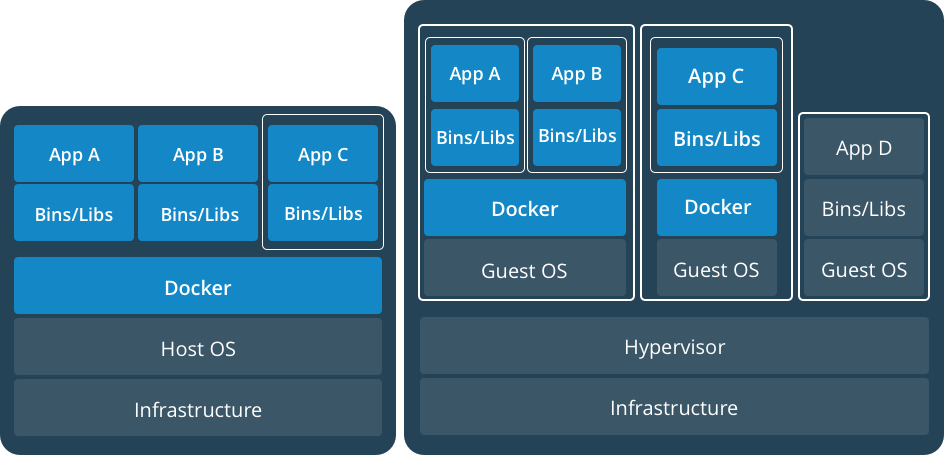
\includegraphics[width=\textwidth]{img/vm-container}
    \caption{Différences entre virtualisation et conteneurs}
    \label{fig:diffvm}
\end{figure}

Cela donne l'avantage aux conteneurs d'être plus rapide et léger car stocker et émuler un noyau
et un système d'exploitation demande plus d'espace disque, de mémoire vive et de puissance de
calcul. Enfin cette légereté font que les conteneurs sont plus facilement déployable.

Cependant à la différence d'une machine virtuelle, ce n'est pas une isolation complète, et donc
si l'application est critique est nécessite un fort niveau d'isolation, mieux vaut utiliser une
machine virtuelle.\newline

Il existe également une bibliothèque d’images publics, le \emph{Docker Hub}, permettant de
récupérer et de créer des images pour facilement créer tous types de conteneurs.

\subsection{Swarm}

Docker Swarm est un outil d’orchestration permettant de créer et gérer des clusters de machines
physiques ou virtuelles hébergeant une application. C’est un outil intégré à Docker depuis sa
version 1.12.

Contrairement à l'outil \emph{Docker Compose} qui permet de gérer plusieurs conteneurs sur une même
machine hôte, \emph{Docker Swarm} peut gérer plusieurs machines différentes et des conteneurs sur
différents hôtes.

Un cluster est un ensemble de machines, physiques ou virtuelles, regroupés afin d'en faciliter la
gestion et dépasser les capacités d'une seule machine.

L’interêt principal d’un cluster Swarm est la haute disponibilité que cela procure pour
l’application.

\begin{figure}[h!]
    \centering
    
\includegraphics[width=0.4\textwidth]{img/swarm}
\end{figure}

\section{Fonctionnement interne}

Dans un cluster Swarm, les éléments du cluster sont appelés les \emph{nodes} (noeuds).
Chaque noeud peut être soit un manager, soit un worker.

Un \emph{manager} est une node qui s'occupe de la gestion des permissions, de l'attribution des
tâches et de l'équilibrage de charge.

Un \emph{worker} est une node qui effectue les tâches attribués par le manager.

Il est possible pour un même noeud d’endosser les deux rôles simultanément.

\begin{figure}[h!]
    \centering
    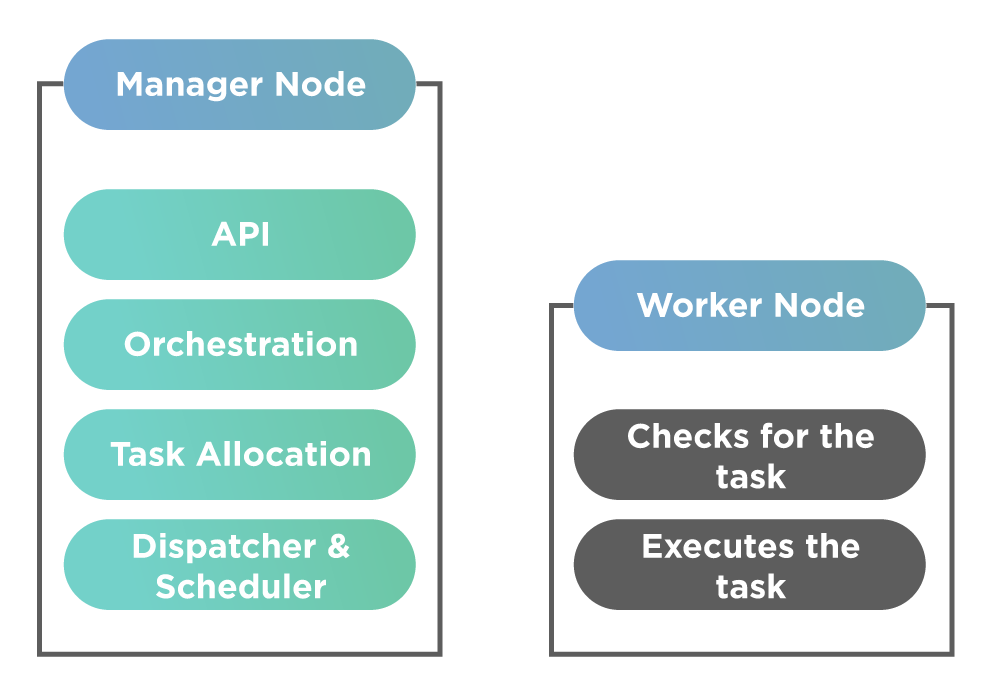
\includegraphics[width=0.5\textwidth]{img/manager}
\end{figure}

Il doit y avoir également dans un cluster une node, plus précisement un manager, qui a le statut de
\emph{leader}. Ce leader s'occupe de la gestion du cluster Swarm et des décisions d'orchestrations.

Swarm est une technologie de clustering qui fonctionne avec agent. C'est via le démon
\verb:dockerd: que les nodes communiquent en utilisant l'API de Docker. Il faut donc installer
Docker, ou à minima le démon sur chacun des noeuds.

\begin{figure}[h!]
    \centering
    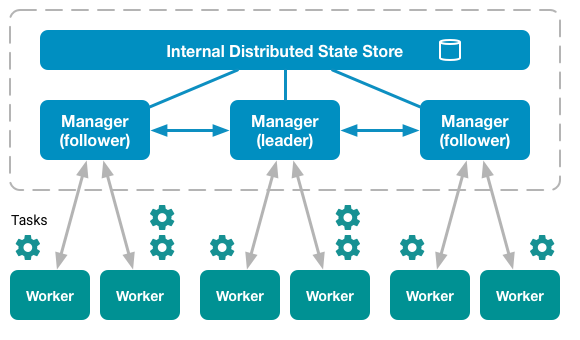
\includegraphics[width=0.8\textwidth]{img/swarm-network}
    \caption{Schéma de fonctionnement d'un cluster Swarm}
\end{figure}

\subsection{Raft Consensus algorithm}

Lorsque Docker fonctionne en mode cluster avec Swarm, les managers utilise l'algorithme du
\href{https://raft.github.io/}{\emph{Raft Consensus}} afin de garantir le fait qu'il partage le
même état du cluster. C'est pour cela que parmi les managers, il y aura un noeud qui sera élu
\emph{leader}.\newline

Cette algorithme permet d'élire un leader afin que celui puisse notifier les autres quant aux
changements d'états du cluster. Si le leader s'arrête l'algorithme est prévu pour un élire un
nouveau de manière automatique. Cette algorithme a l'avantage d'être simple et efficace et il
peut tolérer jusqu'à $(N - 1) / 2$ erreurs, N étant le nombre de noeuds du cluster.

\begin{figure}[h!]
    \centering
    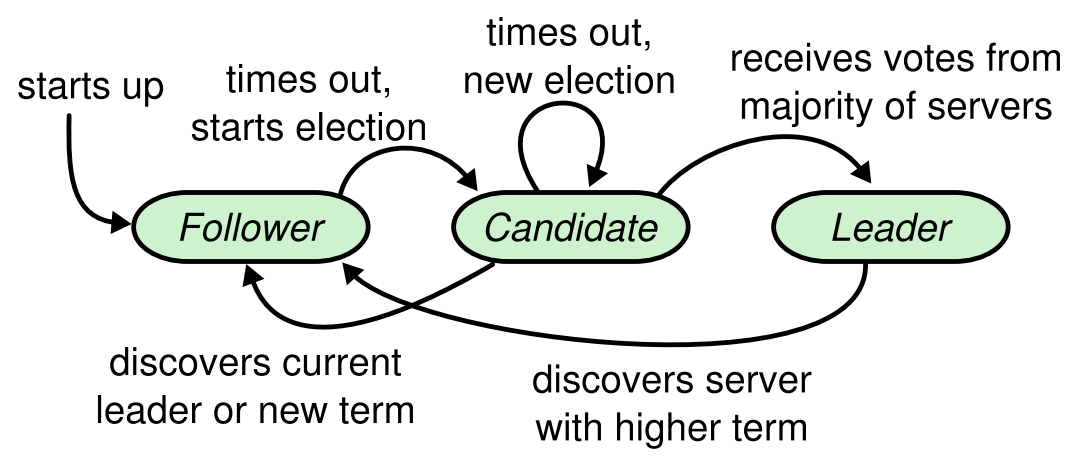
\includegraphics[width=0.8\textwidth]{img/raft}
    \caption{Schéma de fonctionnement de l'algorithme Raft Consensus}
\end{figure}

Afin de mieux comprendre le fonctionnement de cet algorithme, un page l'expliquant simplement
est disponible au lien suivant : 
\href{http://thesecretlivesofdata.com/raft/}{http://thesecretlivesofdata.com/raft/}.

\chapter{Interêts}

\section{Interêt du clustering}

L'utilisation du clustering fourni principalement 2 avantages considérables par rapport à
l'utilisation de machines indépendantes.\newline

Premièrement, la \emph{disponibilité}, l'application sera toujours accessible, car même si un des
serveurs tombent en panne alors qu'il était en train d'exécuter une tâche, un autre peut prendre
le relais. Le seul cas ou l'application pourraît être indisponible serait que tous les serveurs
tombent en panne en même temps, ce qui est peu probable.\newline

Ensuite, l'\emph{évolutivité}, si l'application grandit ou que son utilisation croît beaucoup
il est très simple d'ajouter un ou plusieurs noeuds au cluster afin d'augmenter ses capacités,
sans même stopper le service.

\section{Pourquoi utiliser Docker Swarm ?}

Docker Swarm présente plusieurs avantages :
\begin{itemize}
    \item \emph{Intégration à Docker} : si Docker est déjà la technologie utilisé pour un service,
        il sera très de passer à du clustering.

    \item \emph{Scalabilité} : il est très simple d'ajouter ou de retirer des noeuds afin d'ajuster
        ce nombre à la charge du service.

    \item \emph{Retour à l'état souhaité} : le manager du cluster fait toujours en sorte de faire
        correspondre l'état actuel à celui demandé. Par exemple si le cluster utilise 10 clones
        d'un conteneur afin de fournir le service et que 2 d'entre eux échouent, le manager va
        recréer 2 clones afin de retourner à l'état demandé.

    \item \emph{Réseau multi-hôtes} : un cluster peut utiliser des machines sur plusieurs réseaux
        différents.

    \item \emph{Équilibrage de charge automatique} : pour un service, l'équilibrage est automatique
        entre les noeuds. Il est cependant possible d'utiliser un équilibreur de charge externe.
    
    \item \emph{Sécurité} : la communication entre chacun des noeuds est sécurisée en utilisant
        du chiffrement et une authentification mutuelle avec TLS. On peut utilisé des certificats
        auto-signés ou utiliser une autorité de certification personalisée.
\end{itemize}

\chapter{Installation}

\section{Linux}

Swarm est intégré à Docker par défaut, il suffit donc d'installer le Docker Engine.
Sous Linux, l'installation est très simple et se résume au téléchargement des paquets suivants :

\begin{bashWithTitle}{Ubuntu / Debian}
sudo apt install docker-ce docker-ce-cli containerd.io docker-compose-plugin
\end{bashWithTitle}

\begin{bashWithTitle}{CentOS}
sudo yum install docker-ce docker-ce-cli containerd.io docker-compose-plugin
\end{bashWithTitle}

\begin{bashWithTitle}{Fedora}
sudo dnf install docker-ce docker-ce-cli containerd.io docker-compose-plugin
\end{bashWithTitle}

\begin{bashWithTitle}{Arch Linux}
sudo pacman -S docker docker-compose
\end{bashWithTitle}

\emph{Source} :
\href{https://docs.docker.com/engine/install/}{https://docs.docker.com/engine/install/}

\section{Windows \& MacOS}

Sur Windows et MacOS l'installation est différente car Docker est basé sur les conteneurs LXC.
Il faut donc l'installer sur une machine virtuelle Linux, ou bien installer \emph{Docker Desktop}
qui est une application de bureau fournissant une VM légère intégré. Elle permet donc de créer
et d'utiliser les conteneurs Docker sous Windows et MacOS.\newline

Pour installer cette application il suffit de télécharger l'installeur correspondant sur le site
de Docker : \href{https://www.docker.com/products/docker-desktop/}{https://www.docker.com/products/docker-desktop/}.

\begin{itemize}
    \item[•] Windows : \verb:Docker Desktop Installer.exe:
    \item[•] MacOS : \verb:Docker.dmg:
\end{itemize}

Cette application possède plus de fonctionnalités que l'interface en ligne de commande, et est plus
simple à utiliser pour un utilisateur novice, il est donc aussi possible de l'installer sur Linux
si l'on souhaite.

\chapter{Utilisation}

\section{Commandes de bases}

Les commandes du mode \verb:swarm: de docker sont les suivantes:
\begin{itemize}
	\item \verb:swarm init:: Initialise un \verb:swarm:. Le nœuds docker ciblé par 
        cette commande devient un manager pour un nouveau \verb:swarm: initialement vide.
	\item \verb:swarm join:: Permet à un nœuds docker de rejoindre un \verb:swarm: existant
        en indiquant le token fournis par la commande \verb:swarm init:.
    \item \verb:swarm leave:: Permet à un nœud de quitter le \verb:swarm:, pour retirer un 
        manager de l'essain il faut utiliser l'option \verb:--force:.
\end{itemize}

\section{Un cas d'utilisation}

On va maintenant mettre en place un \verb:swarm: avec un manager et deux workers. Afin de
simuler un réseau de plusieurs machines on va installer \verb:docker: sur des conteneurs
lxc en utilisant le script d'installation fournis en annexe. Le montage réseau est le suivant:
\begin{bash}
NAME           STATE            IPV4        
docker-manager RUNNING 10.0.3.111, 172.17.0.1
docker-worker1 RUNNING 10.0.3.235, 172.17.0.1
docker-worker2 RUNNING 10.0.3.203, 172.17.0.1
\end{bash} 
\begin{center}
    \emph{Les adresses \verb:172.17.0.1: correspondent à l'interface docker0}
\end{center}
\jmp

On commence donc par créer un \verb:swarm: depuis le conteneur du manager:
\begin{bash}
docker swarm init
Swarm initialized: current node (qt9wx5u1hegtv8mjg61zbxnob) is now a manager.
To add a worker to this swarm, run the following command:
    docker swarm join --token SWMTKN-1-5oug0mpki7... 10.0.3.111:2377
\end{bash}
On note le token afin de pouvoir l'utiliser plus tard. On peut vérifier le status de 
ce nœud avec la commande \verb:docker node ls: qui produit la sortie suivante:
\begin{bash}
ID                        HOSTNAME         STATUS    AVAILABILITY   MANAGER
qt9wx5u1hegtv8mjg61zbxnob docker-manager   Ready     Active         Leader
\end{bash}
Ce qui confirme bien que l'essaim à été créé. On va maintenant ajouter les deux worker à notre 
essaim, on se connecte sur chacun des conteneurs et on utilise la commande suivante:
\begin{bash}
docker swarm join --token SWMTKN-1-5oug0mpki7... 10.0.3.111:2377
This node joined a swarm as a worker.
\end{bash}
Si on se reconnecte sur le conteneur du manager et que l'on lance à nouveau la commande
\verb:docker node ls:, on peut voir que l'essaim comporte bien 3 machines:
\begin{bash}
ID                          HOSTNAME         STATUS    AVAILABILITY   MANAGER
qt9wx5u1hegtv8mjg61zbxnob * docker-manager   Ready     Active         Leader 
u2g1r24whkfz34mwn8rb9ovrs   docker-worker1   Ready     Active                
73t7ozstyb7d312888879i6um   docker-worker2   Ready     Active                
\end{bash}
On doit à présent déployer un service sur notre essaim. On va utiliser dans pour cette exemple
le cas d'un service web dont on souhaite répartir la charge sur les 3 conteneurs. On va pour cela
utiliser le serveur web \verb:nginx:. On lance la commande suivante depuis le manager 
pour créer un service web répartis entre les conteneurs:
\begin{bash}
docker service create --name my_web --replicas 3 --publish 8080:80 nginx
\end{bash}
\begin{itemize}
    \item \verb:--name:: permet d'indiquer le nom de ce service.
    \item \verb:--replicas:: indique le nombre de nœuds de l'essaim auquel on souhaite
        attribuer cette tâche, ici 3.
    \item \verb:--publish:: permet d'indiquer que l'on souhaite rediriger tous le traffic 
        entrant sur le port 8080 du conteneur lxc sur le port 80 du service docker.  
\end{itemize}
Il est important de noter que l'option \verb:--publish: en plus de faire la redirection,
active le mode \verb:routing mesh:. Ce mode permet de faire de l'équilibrage de charge de
manière transparente pour le client, en effet une requête effectué sur un nœud de l'essaim 
peut être traité par un autre nœud si le premier nœud est indisponible.\newline 

Pour l'instant on peut vérifier que le service \verb:my_web: fonctionne sur l'ensemble des
nœuds de l'essaim, pour cela on utilise la commande suivante:
\begin{bash}
docker service ps my_web
ID           NAME     IMAGE        NODE           DESIRED STATE
8z15jsh81yzb my_web.1 nginx:latest docker-manager Running      
wbh4bodsezqa my_web.2 nginx:latest docker-worker1 Running      
ou5pyyrpr6k1 my_web.3 nginx:latest docker-worker2 Running       
\end{bash}
\newpage

Il est possible de se connecter sur l'une des interfaces web en allant par exemple sur 
\url{http://10.0.3.111:8080/}

\begin{figure}[h!]
    \centering
    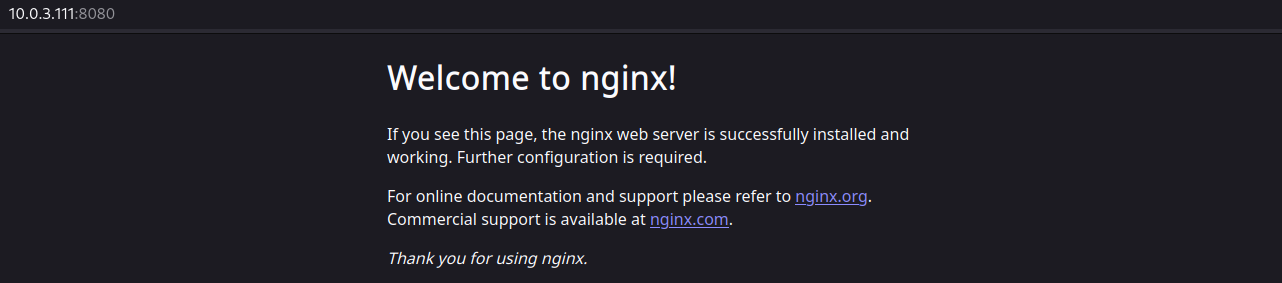
\includegraphics[width=\textwidth]{img/nginx}
    \caption{Page par défault de nginx}
\end{figure}

\chapter{Configuration}

\section{Performances}



\section{Sécurité}

En terme de sécurité Docker Swarm propose principalement deux fonctionnalités :\newline

Premièrement, Docker possède un système de PKI (Public Key Infrastructure) intégré.
Lors de la création du cluster (à la commande \verb:docker swarm init:), le noeud est
alors déclaré comme manager. Ensuite le manager va généré une nouvelle autorité de 
certification en utilisant le PKI, ce qui permettra ensuite de générer des certificats pour
chacun des noeuds qui rejoindra le cluster.

Ces certificats seront ensuite utilisé pour chiffrer et authentifier les communications
entre les noeuds en utilisant TLS (Transport Layer Security). Si l'on souhaite on peut
fournir à Swarm une autorité de certification externe plutôt que d'utiliser celle interne
à Docker.\newline

Ensuite, Swarm chiffre également par défaut les logs du Raft Consensus afin de protéger
la configuration et les données d'éventuels attaquants. Les clés utilisés pour chiffrer les
logs et pour utiliser TLS sont chargées dans la mémoire du noeud au démarrage ou au
redémarrage. Cependant afin de protéger ces clés lorsque le service est éteint, Docker propose
la fonctionnalité d'\verb:autolock:.

Ce paramètre a pour effet de chiffrer le contenu des noeuds lorsque le service s'arrête, il
faudra donc fournir une clé de déchiffrement au redémarrage du service. Cette clé est donné lors
de la création du Swarm avec l'option \verb:autolock: ou bien si l'on active l'option sur un
cluster existant.\newline

Dans la pratique il faut utiliser les commandes suivantes pour activer la fonctionnalité :

\begin{bashWithTitle}{À la création :}
docker swarm init --autolock
\end{bashWithTitle}

\begin{bashWithTitle}{Sur un cluster existant :}
docker swarm update --autolock=true
\end{bashWithTitle}
\newpage

Ces commandes vont nous renvoyer une clé de la forme :
\begin{bash}
SWMKEY-1-WuYH/IX284+lRcXuoVf38viIDK3HJEKY13MIHX+tTt8    # Exemple
\end{bash}

Au redémarrage on pourra déverrouiller le cluster avec la commande suivante, en fournissant la clé
précédente :
\begin{bash}
docker swarm unlock
\end{bash}

\emph{Source} : \href{https://docs.docker.com/engine/swarm/swarm\_manager\_locking/}{https://docs.docker.com/engine/swarm/swarm\_manager\_locking/}

\section{Disponibilité}

Si on arrête le conteneur lxc \verb:docker-worker1:, puis que l'on se connecte sur le
conteneur du manager afin d'afficher l'état de l'essaim on obtient ceci:

\begin{bash}
docker service ps my_web
ID           NAME         IMAGE        NODE           DESIRED STATE   
8z15jsh81yzb my_web.1     nginx:latest docker-manager Running         
41hbyfhleu1l my_web.2     nginx:latest docker-worker2 Running        
wbh4bodsezqa  \_ my_web.2 nginx:latest docker-worker1 Shutdown      
ou5pyyrpr6k1 my_web.3     nginx:latest docker-worker2 Running      
\end{bash}

On peut voir que le conteneur docker-worker2 à récupèrer la tâche du worker1 de manière
autonome et transparente, ce qui veut dire qu'en cas de panne ou autre indisponibilité, 
docker équilibre automatiquement la charge.


\chapter{Conclusion}
